\chapter{Materialien}
\label{cha:materials}

Dieses Kapitel befasst sich mit den in dieser Bacherlorarbeit verwendeten Materialien. Dazu gehört die Hardware und die Software.

\section{ZedBoard development kit}
\label{sec:basics_zedboard}

Das ZedBoard von Digilent ist ein Entwicklungs- und Evaluationsboard mit einem verbauten Xilinx Zynq-7000 \gls{SoC} mit Peripherie. 
Das Zynq \gls{SoC} ist in 3 Blöcke aufgeteilt, wie in \cref{fig:zedboard_block_diagram} detailliert aufgeführt ist:

\begin{easylist}[itemize]
	& \gls{MIO}
	& \gls{PS}
	& \gls{PL}
\end{easylist}

Das \gls{PS} verfügt über einen \gls{ARM}-Cortex\texttrademark A9 Prozessor und kann auf den \gls{DDR SDRAM} zugreifen.
Das \gls{PL} stellt ein \gls{FPGA} mit Peripherie dar und kann sowohl als domänenspezifischer Beschleuniger für das \gls{PS} als auch als eine autarke Einheit konfiguriert werden.
Das \gls{MIO} fasst die sowohl von der \gls{PS} als auch \gls{PL} nutzbare Peripherie - exklusiver Zugriff vorausgesetzt - zusammen. 

%Aus dieser Struktur wird ersichtlich, dass ein Zugriff auf sämtliche Ressourcen aus der \gls{PL} nicht ohne Weiteres möglich ist. \cite[16]{article:plasma_mips_processor} Dazu gehören unter Anderem der \gls{DDR SDRAM}, der SD-Kartenleser sowie der \gls{UART}-Controller. Ein Zugriff auf diese ist in der einfachsten Variante nur über das Einrichten und Hochfahren des \gls{PS} mit dem integrierten \gls{ARM}-Prozessor und eines vollwertigen Betriebssystems möglich, was der Umsetzung einer eigenen \gls{CPU} bzw. \gls{SoC} nicht gerade dienlich ist. Einige Einschränkungen lassen sich durch den Einsatz der \glspl{PMOD} umgehen. Es wurden Module für \gls{USB}-\gls{UART} erworben, sowie ein SD-Kartenleser-Modul. Wie in \cref{fig:zedboard_block_diagram} dargestellt, sind die \glspl{PMOD} auch von der \gls{PL} ansprechbar und somit nutzbar.
%
%Auf dem ZedBoard sind unter Anderem auch ein Display-Modul, ein \gls{HDMI}-Transmitter sowie ein \gls{VGA}-Ausgang verbaut. Diese sind ausschließlich von der \gls{PL} aus ansprechbar.

\begin{figure}[!htbp]
	\centering
	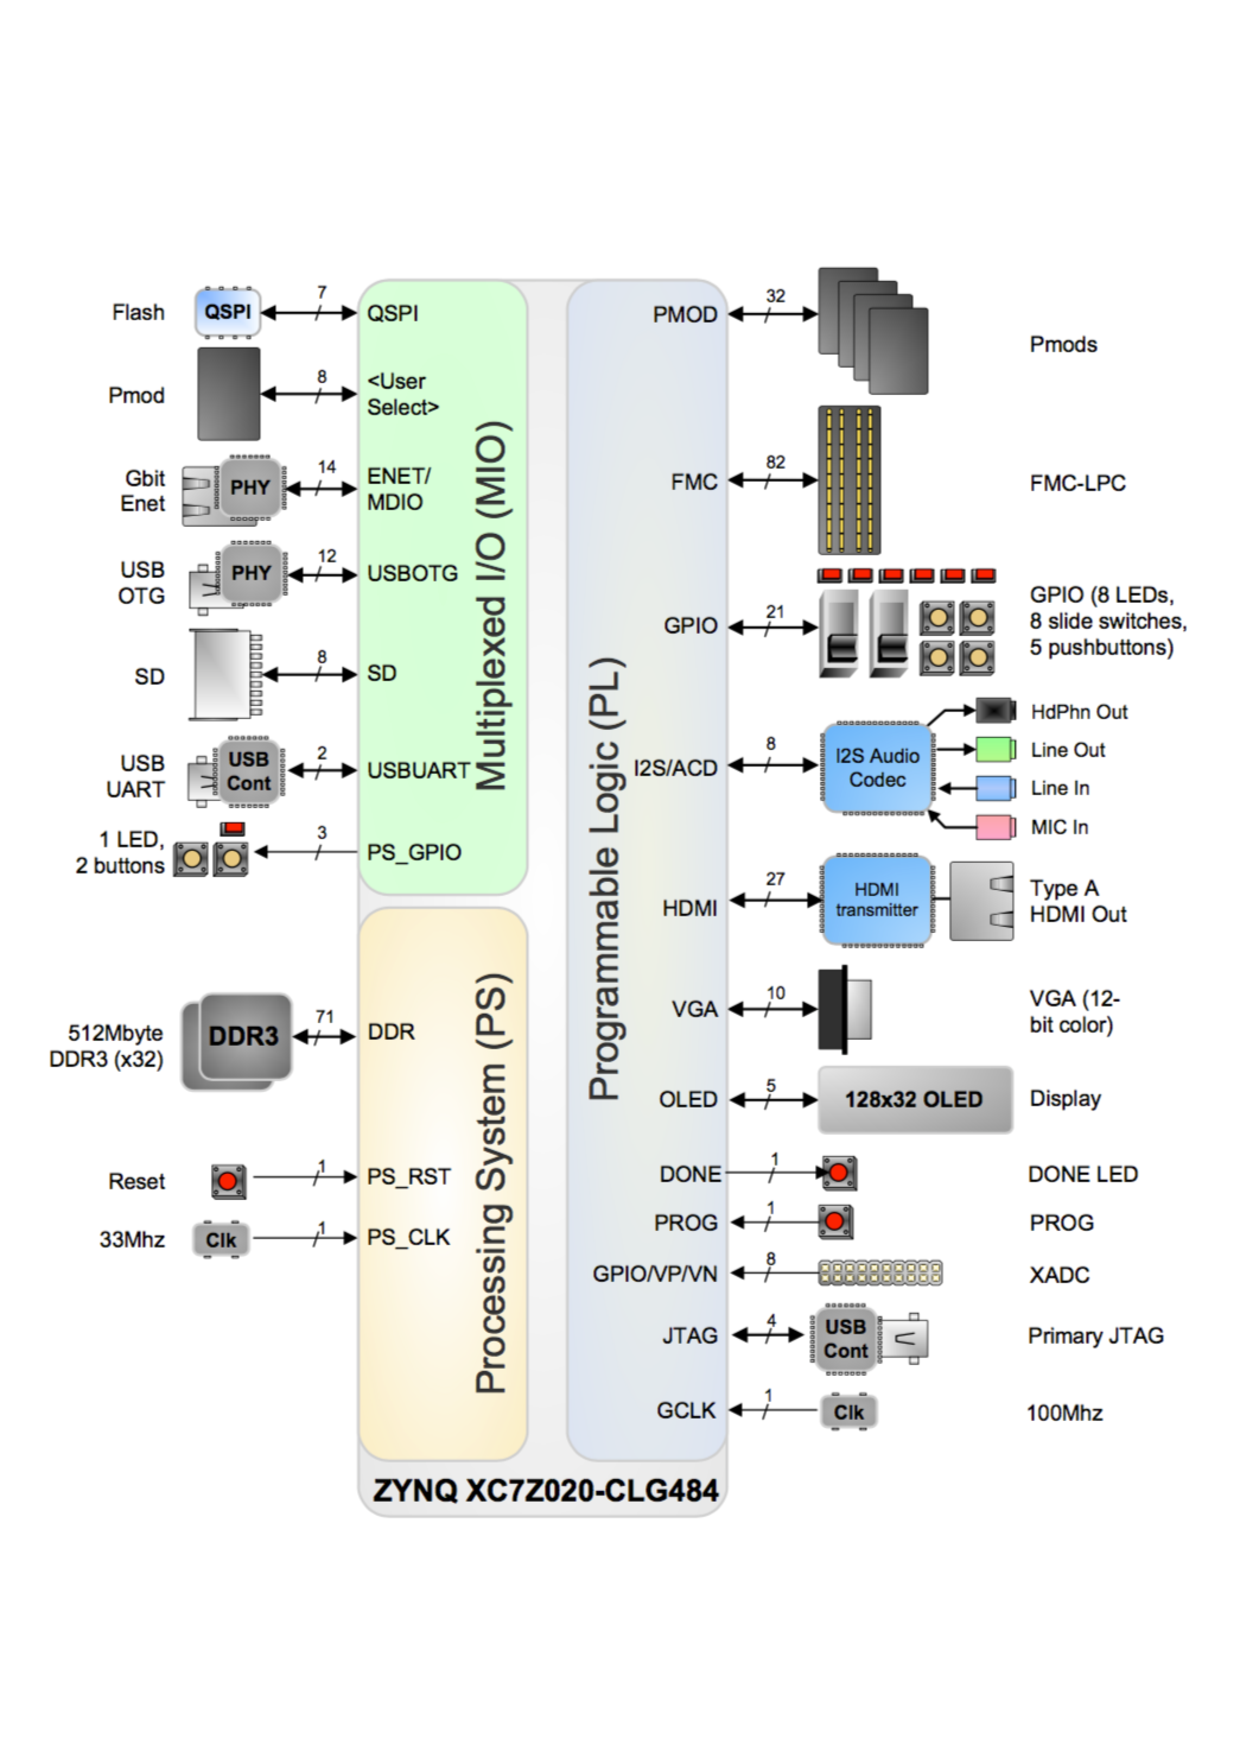
\includegraphics[width=0.6\linewidth]{images/zedboard_block_diagram}
	\caption{ZedBoard Blockdiagramm \cite[3]{manual:zedboard}}
	\label{fig:zedboard_block_diagram}
\end{figure}

\section{DE1-SoC development kit}
\label{sec:basics_de1_soc}

Das DE1-SoC Board von Terasic ist ein Eintwicklungs- und Evaluationsboard mit einem verbauten Cyclone V \gls{FPGA}-\gls{SoC}.

Wenn man das in \cref{fig:de1_soc_block_diagram} abgebildete Blockdiagramm betrachtet und mit dem Blockdiagramm des ZedBoard in \cref{fig:zedboard_block_diagram} vergleicht, so fallen starke Ähnlichkeiten auf. Diese sind darin begründet, dass bei beiden \glspl{FPGA} ein ähnliches Konzebt verfolgt wird, bei dem sowohl ein \gls{ARM}-Prozessor als auch ein \gls{FPGA} mit Peripherie zur Verfügung gestellt wird. Diese Architektur wird in der Altera-Terminologie \enquote{SoC FPGA} bzw. \enquote{SoCFPGA} genannt \cite[1]{manual:socfpga}. 

\begin{figure}[!htbp]
	\centering
	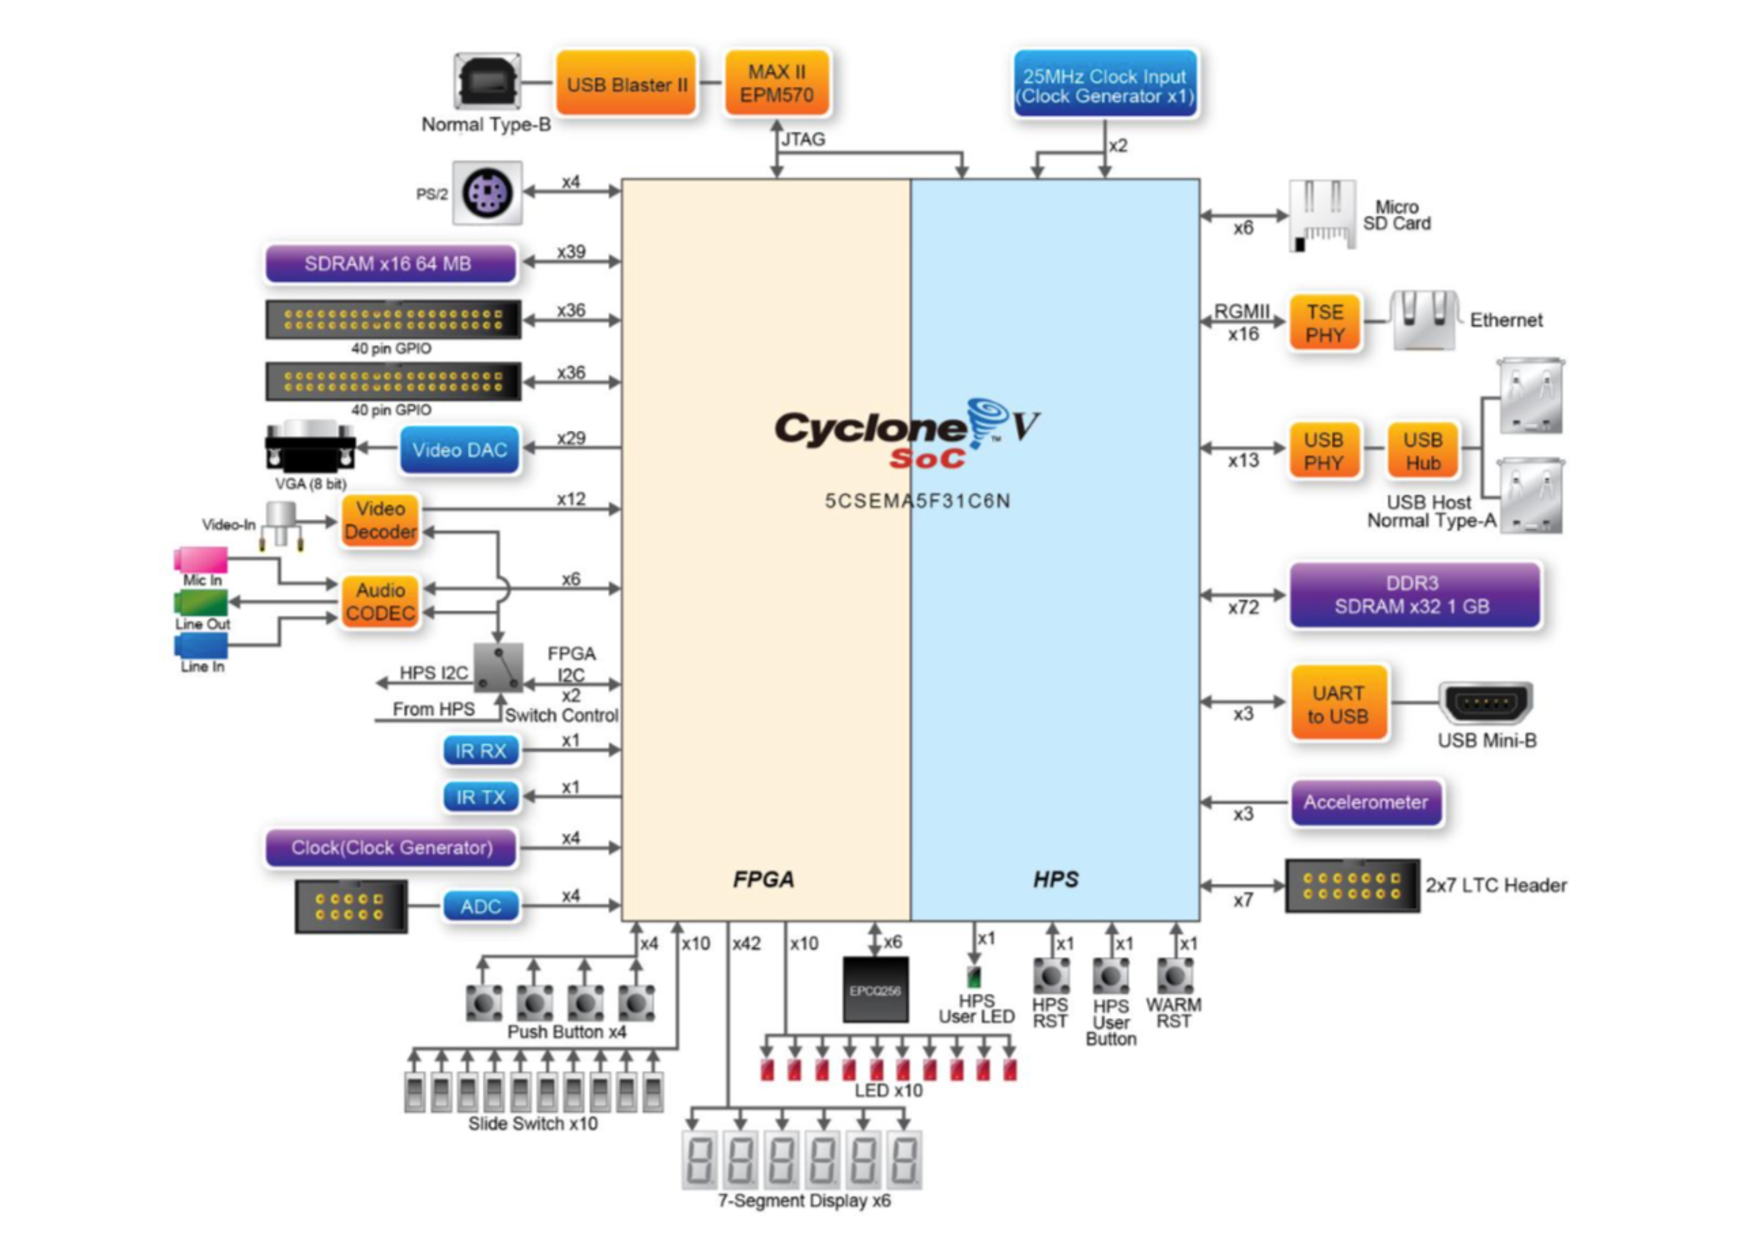
\includegraphics[width=0.7\linewidth]{images/de1_soc_block_diagram}
	\caption{DE1-SoC Blockdiagramm \cite[9]{manual:de1soc}}
	\label{fig:de1_soc_block_diagram}
\end{figure}

Auf dem DE1-SoC-Board stehen folgende Komponenten zur Verfügung \cite{manual:de1soc}:
\begin{easylist}[itemize]
	& \gls{FPGA}
	&& Altera Cyclone\textregistered V SE \gls{FPGA}
	&& \SI{64}{\mega\byte} SDRAM (\SI{16}{bit} Datenbus)
	&& 4 Taster
	&& 10 Schalter
	&& 10 rote LEDs
	&& 6 7-Segment-Anzeigen
	&& 4 \SI{50}{\mega\hertz} Oszillatoren
	&& \SI{24}{bit} Audio-CODEC mit Line- und Mikrofoneingängen und Line-Ausgang
	&& VGA DAC mit VGA-Ausgang
	&& TV Decoder (NTSC/PAL/SECAM) und TV-Eingang
	&& PS/2 Maus-/Tastaturanschluss
	&& Infrarot Sender/Empfänger
	&& Zwei 40-Pin GPIO-Leisten
	
	& \gls{HPS}
	&& \SI{800}{\mega\hertz} Dual-core ARM Cortex-A9 MPCore Prozessor
	&& \SI{1}{\giga\byte} DDR3 SDRAM (\SI{32}{bit} Datenbus)
	&& 1 Gigabit Ethernet PHY mit einem RJ45 Anschluss
	&& 2-Port USB Host, normal Type-A USB Stecker
	&& Micro SD-Kartenschacht
	&& Beschleunigungssensor (I2C)
	&& UART to USB, USB Mini-B Stecker
	&& Warm-Reset und Cold-Reset-Taster
	&& Ein benutzerdefinierte Taster, eine benutzerdefinierte LED
	&& LTC 2x7 Erweiterungsstecker
\end{easylist}

In \cref{fig:de1_soc_view_layout} ist die Ober- und Unterseite des DE1-SoC-Boards mit Hervorhebung der einzelnen Komponenten abgebildet.

\begin{figure}[!htbp]
	\centering
	\begin{subfigure}{.6\textwidth}
		\centering
		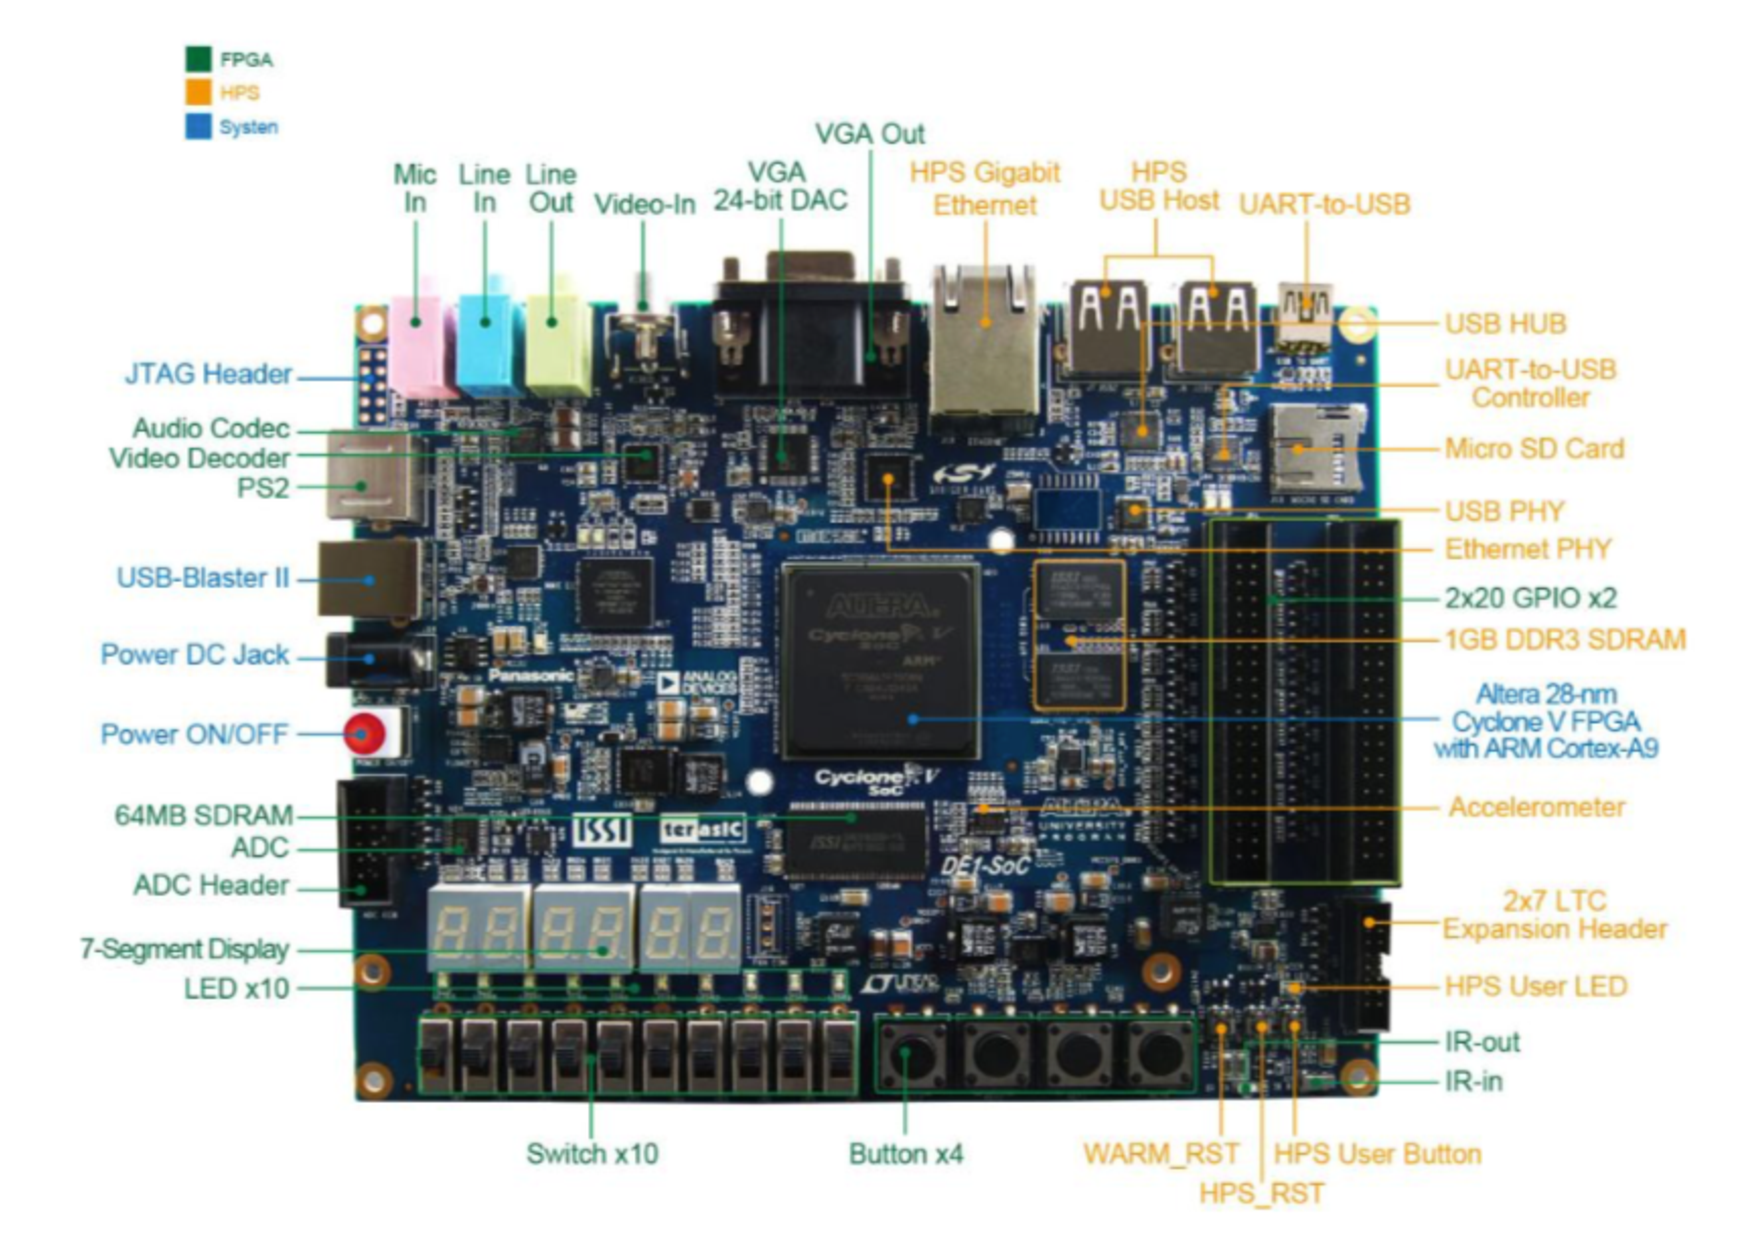
\includegraphics[width=.9\linewidth]{images/de1_soc_view_top}
		\caption{Oberseite}
		\label{fig:de1_soc_view_top}
	\end{subfigure}%
	\begin{subfigure}{.4\textwidth}
		\centering
		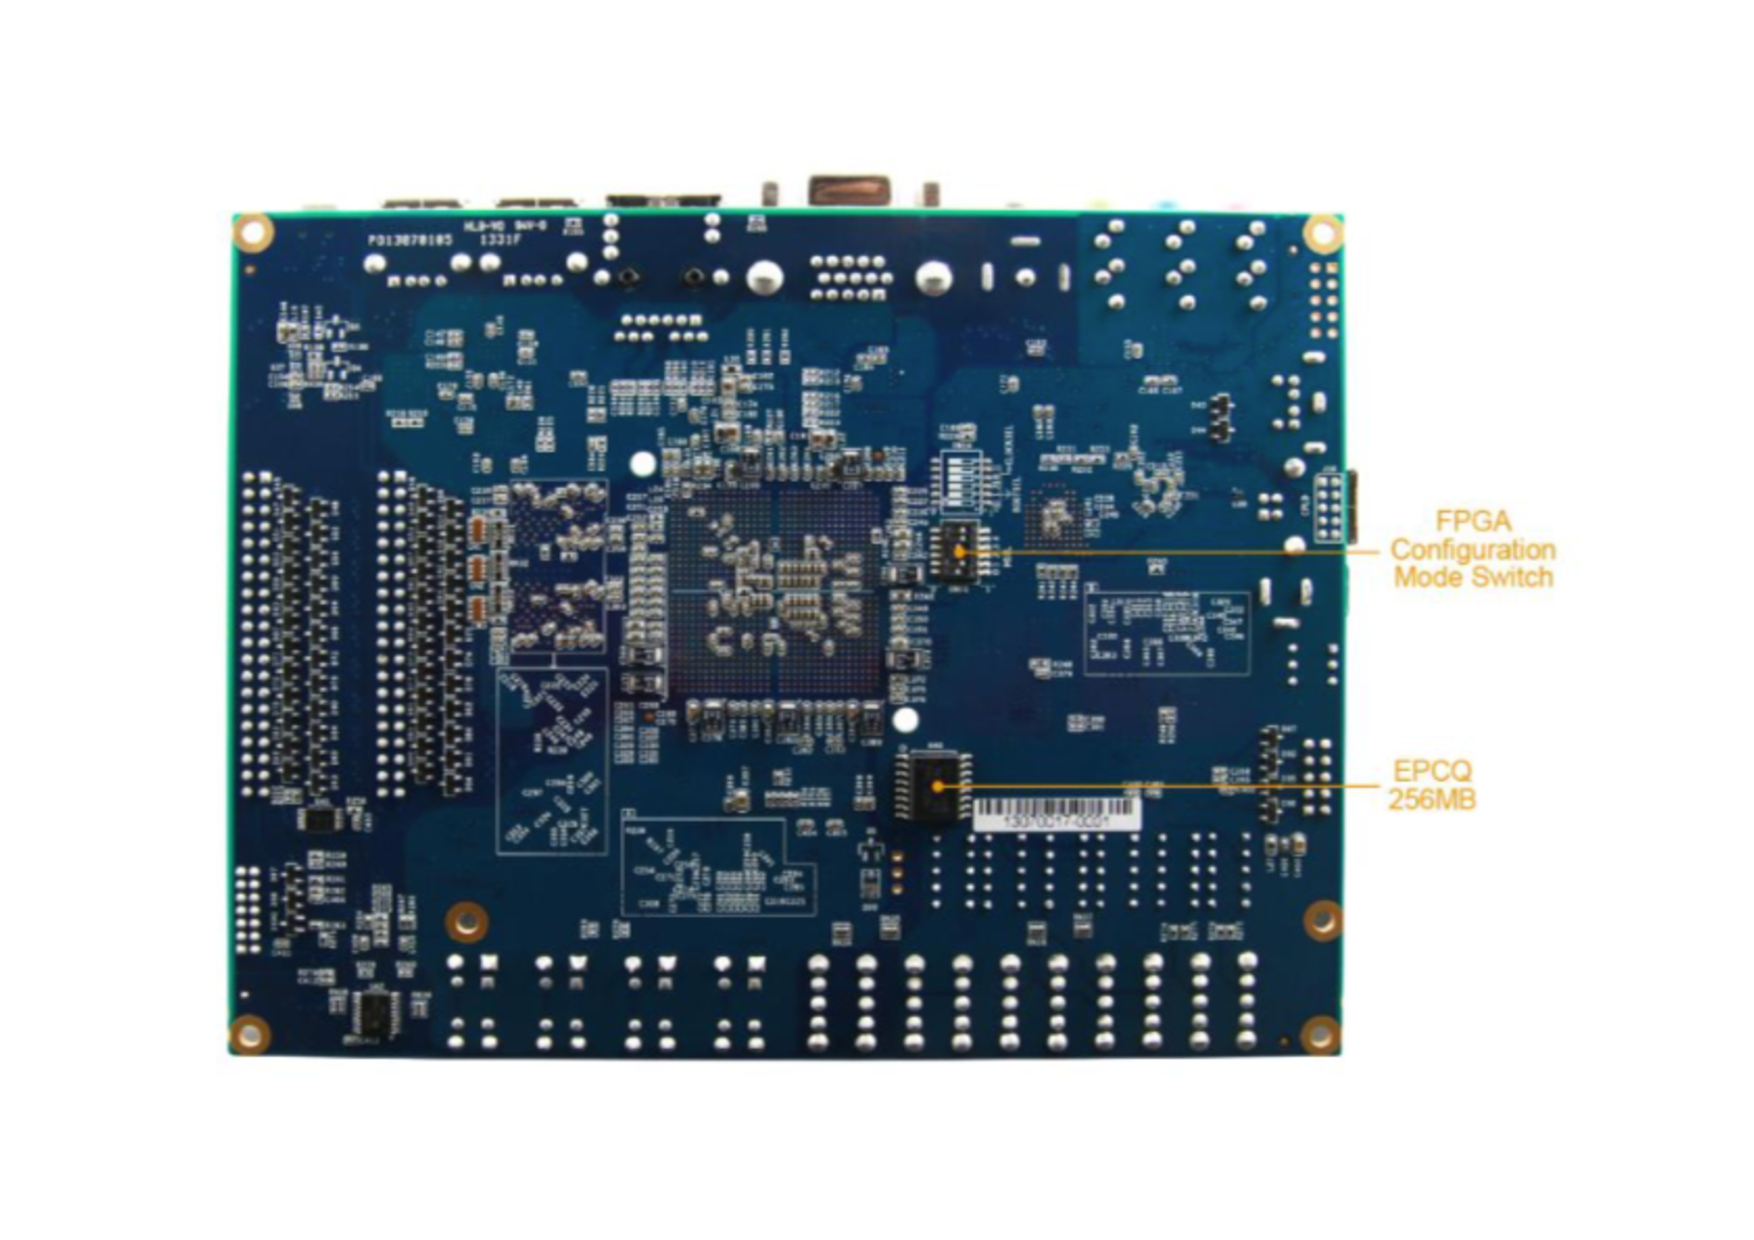
\includegraphics[width=.9\linewidth]{images/de1_soc_view_bottom}
		\caption{Unterseite}
		\label{fig:de1_soc_view_bottom}
	\end{subfigure}
	\caption{DE1-SoC Board-Layout \cite[7]{manual:de1soc}}
	\label{fig:de1_soc_view_layout}
\end{figure}

Zu beachten ist die Einstellung des \enquote{FPGA Configuration Mode Switch} auf der Unterseite des Boards (siehe \cref{fig:de1_soc_msel_switch}). Davon hängt der Konfigurationszeitpunkt des \gls{FPGA} und Programmierbarkeit des \gls{FPGA} zur Laufzeit.

\begin{figure}[!htbp]
	\centering
	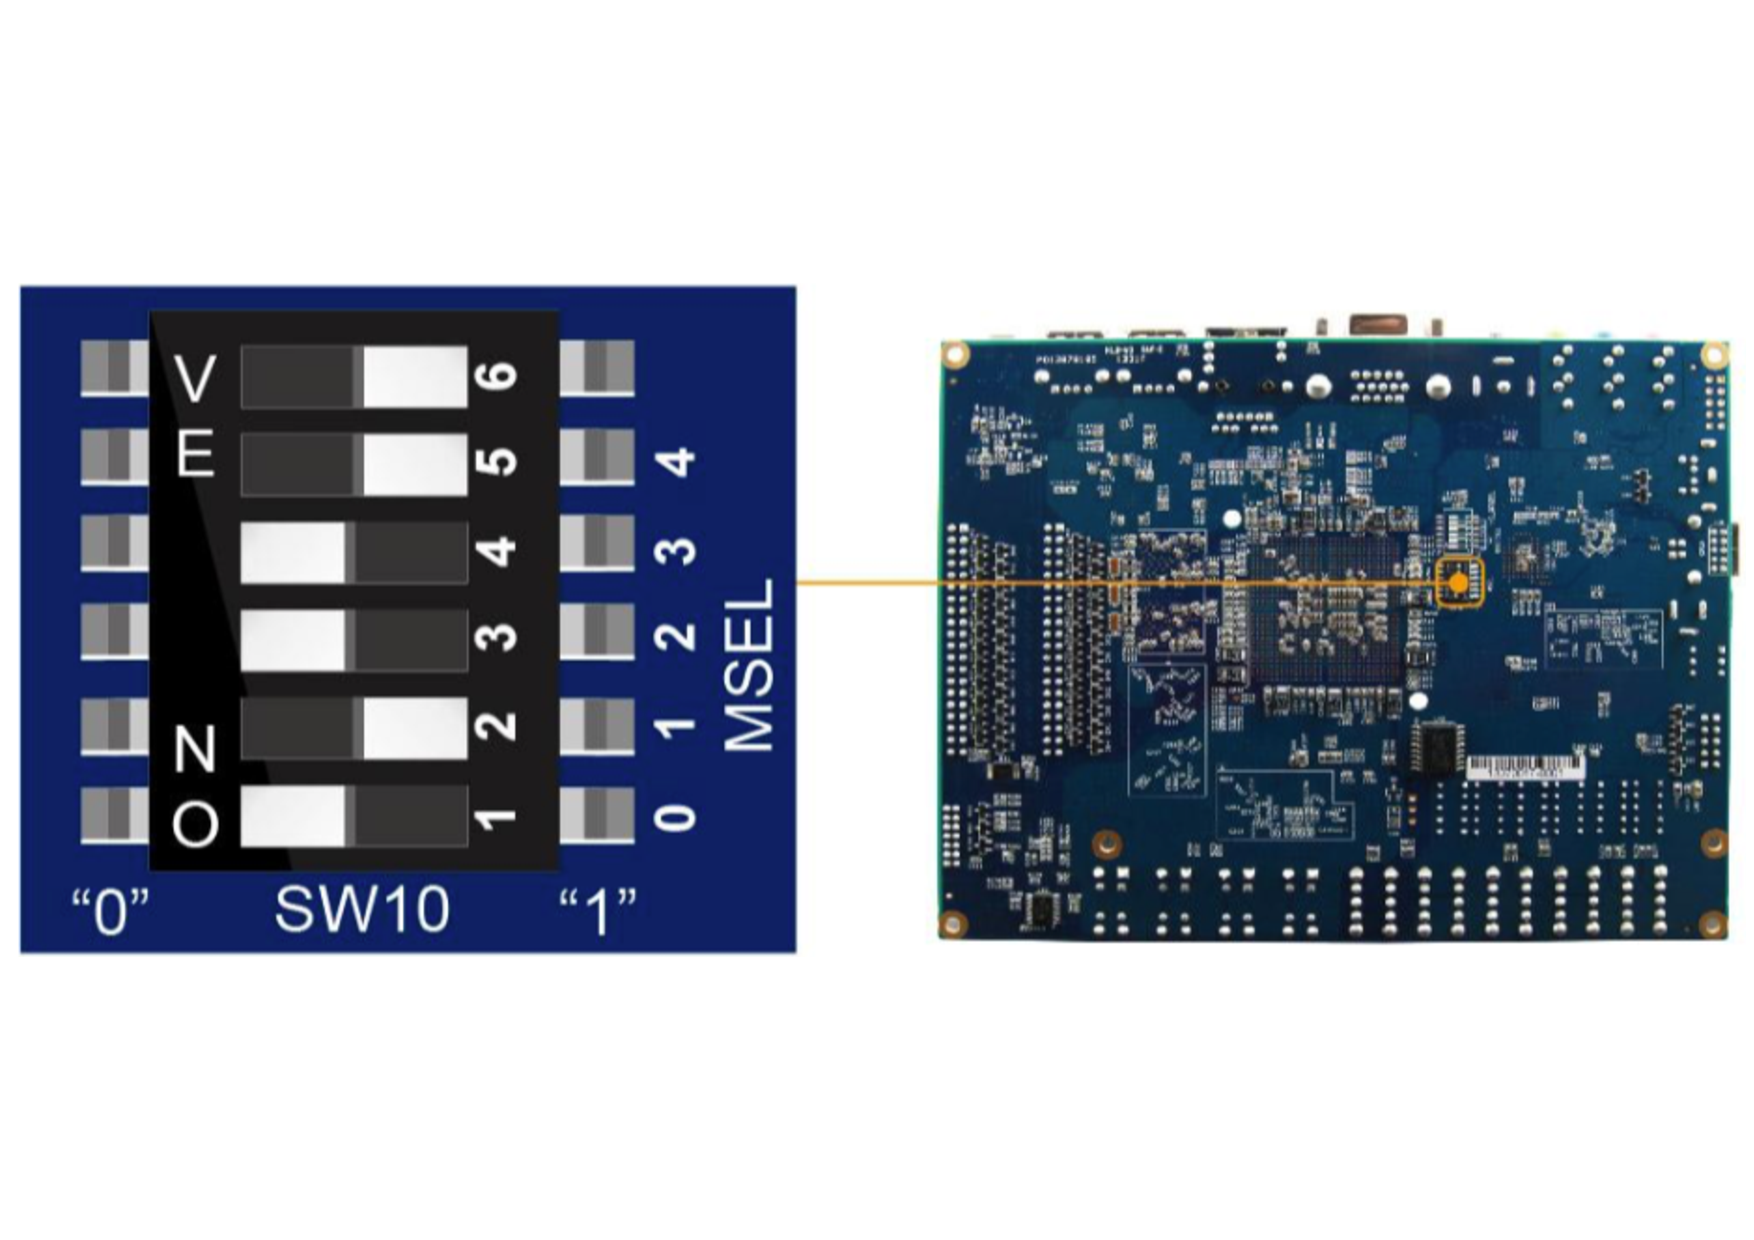
\includegraphics[width=0.7\linewidth]{images/MSEL_config}
	\caption{FPGA Configuration Mode Switch \cite[12]{manual:de1soc}}
	\label{fig:de1_soc_msel_switch}
\end{figure}

\begin{table}[!htbp]
	\bigskip
	\centering
	\begin{tabular}{| l | l | l | }
		\hline
		\textbf{MSEL[4:0]} & \textbf{Konfiguration} & \textbf{FPGA-Konfigurationsquelle} \\
		\hline
		\texttt{10010} & AS & EPCS (Voreinstellung) \\
		\hline
		\texttt{01010} & FPPx32 & \gls{HPS}-Software (Linux) \\
		\hline
		\texttt{00000} & FPPx16 & \gls{HPS}-Software (U-Boot, Abbild auf der SD-Karte) \\
		\hline
	\end{tabular}
	
	\caption{FPGA Konfigurationsmodi \cite[13]{manual:de1soc}}
	\label{tab:de1_soc_msel}
\end{table}

\alertwarning{Eine häufige Fehlerquelle ist eine spiegelverkehrte Einstellung der Konfigurationsschalter, wenn das Board so gehalten wird, dass die PCB-Legenden auf der Unterseite des Boards von links nach rechts gelesen werden können. Die Pin-Belegung ist nicht intuitiv, das MSB befindet sich \textbf{rechts}, und logisch \enquote{1} ist \textbf{unten}}

\section{Quartus Prime 18.0}
Um Hardware für einen \gls{FPGA} entwickeln zu können, bedarf es einer passenden Entwicklungsumgebung. Da dem verwendeten Board ein Altera/Intel \gls{FPGA} zugrundeliegt, wird die Entwicklungsumgebung \enquote{Quartus Prime} verwendet. Diese ist nach einer Registrierung kostenfrei in der Version \enquote{Quartus Prime Lite Edition 18.0} im Downloadportal\footnote{\url{http://fpgasoftware.intel.com/?edition=lite}} von Intel verfügbar. 

In der Entwicklungsumgebung sind mehrere Anwendungen (siehe \cref{fig:quartus_apps}) enthalten, die in dieser Bachelorarbeit verwendet werden:
\begin{easylist}[itemize]
	& Quartus Prime: Wird zur \gls{HDL}-Synthese verwendet
	& Platform Designer: Grafisches \gls{SoC}-Designwerkzeug
	& Signal Tap: Synthetisierbarer Logikanalysator mit grafischer Benutzeroberfläche zur Signaldefinition und Auswertung
	& Modelsim: \gls{HDL}-Simulator
\end{easylist}

\begin{figure}[!htbp]
	\centering
	\begin{subfigure}[b]{0.475\textwidth}
		\centering
		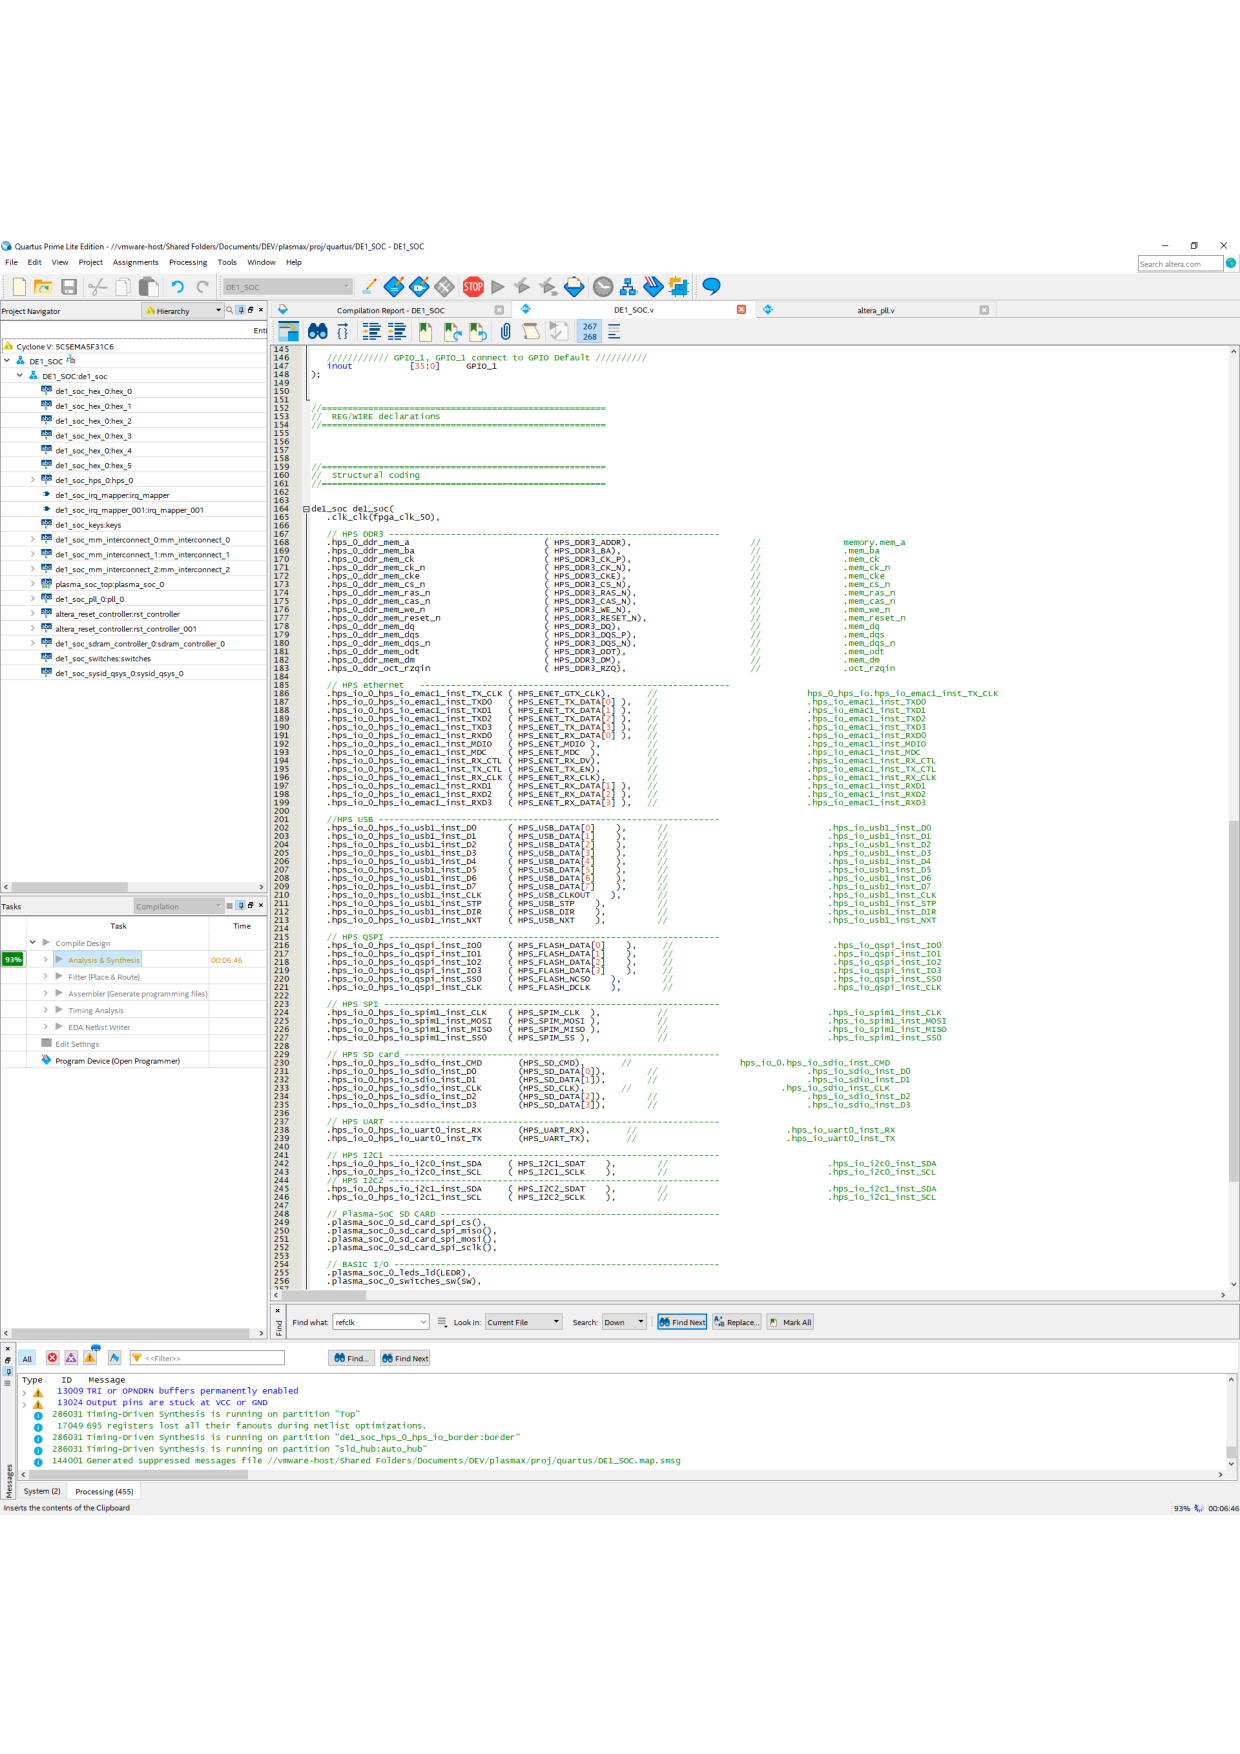
\includegraphics[width=\textwidth]{images/quartus_mainwindow}
		\caption{Quartus}
		\label{fig:quartus_mainwindow}
	\end{subfigure}
	\hfill
	\begin{subfigure}[b]{0.475\textwidth}  
		\centering 
		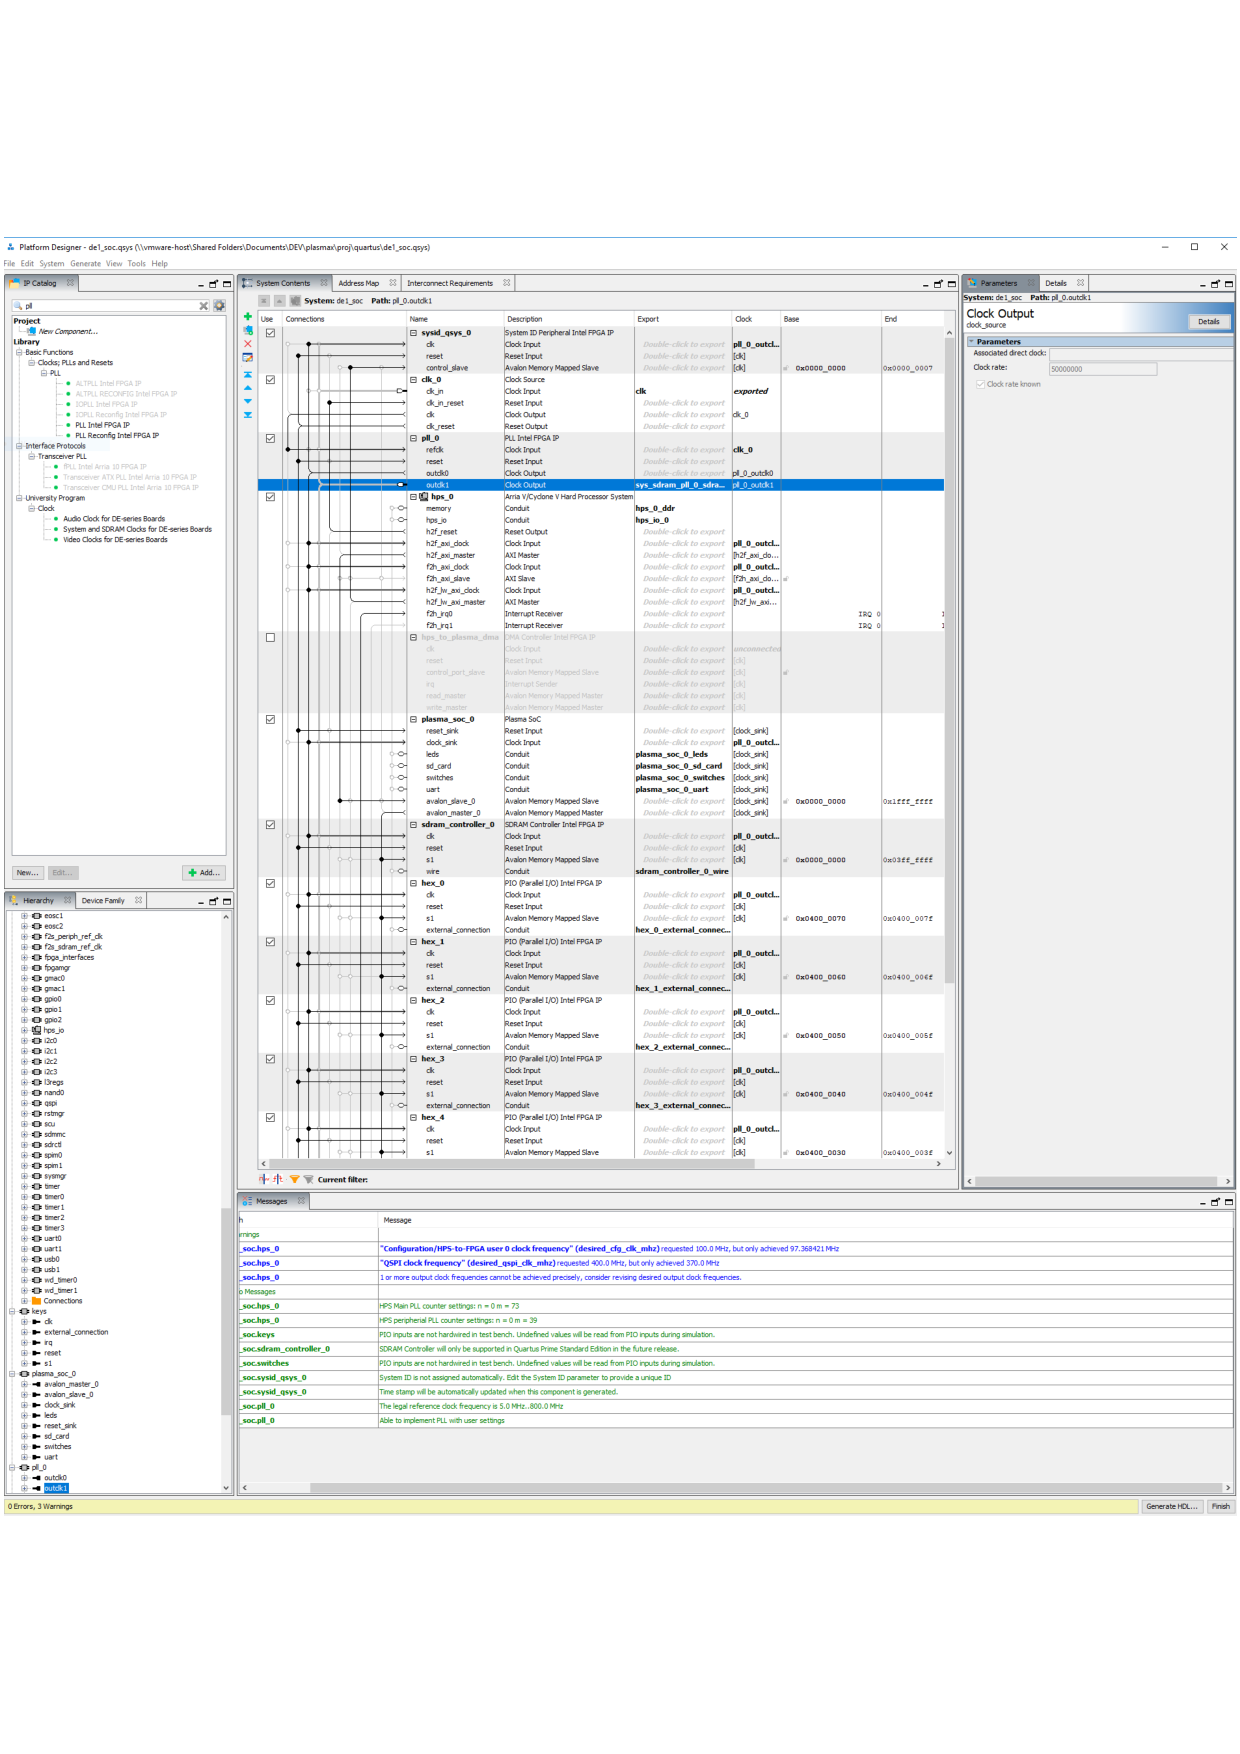
\includegraphics[width=\textwidth]{images/quartus_platformdesigner}
		\caption{Platform Designer}
		\label{fig:quartus_platformdesigner}
	\end{subfigure}
	\vskip\baselineskip
	
	\begin{subfigure}[b]{0.475\textwidth}   
		\centering 		
		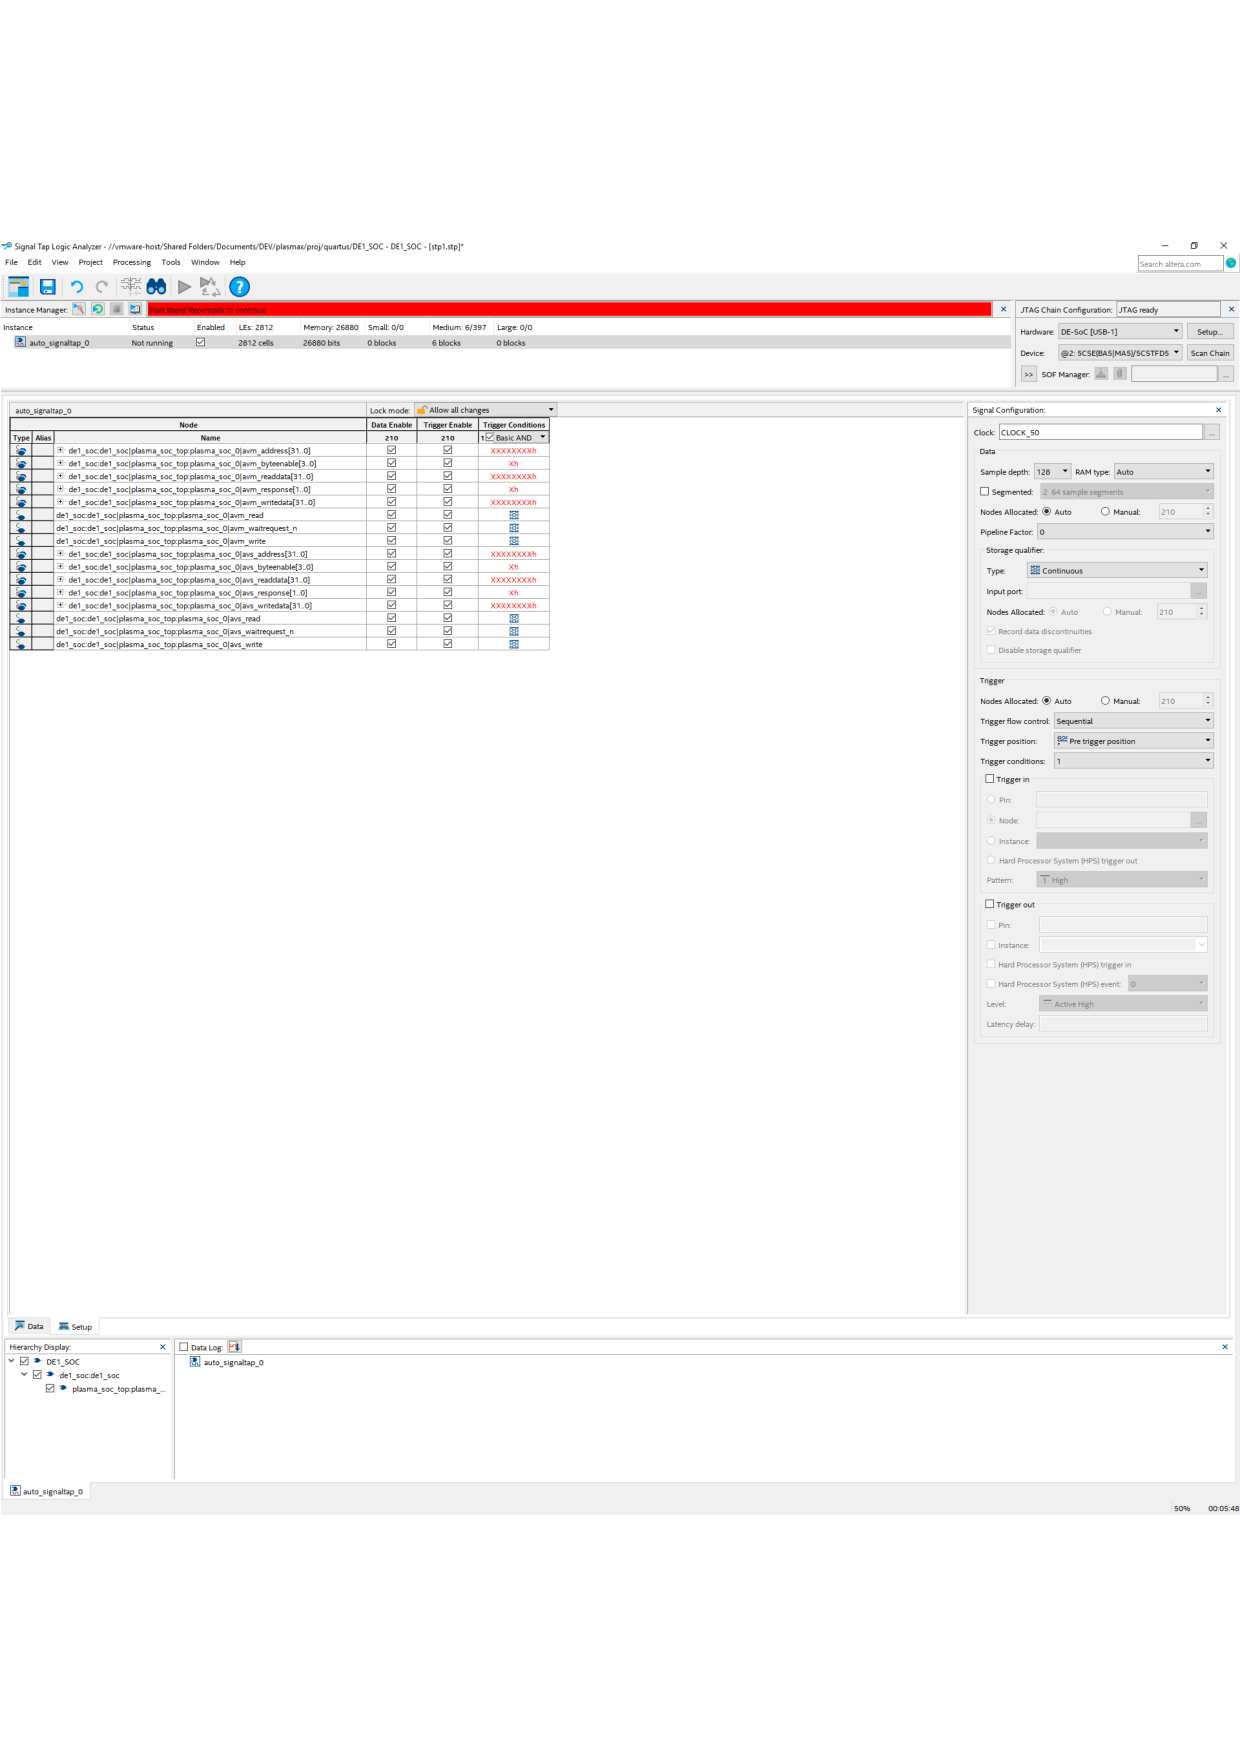
\includegraphics[width=\textwidth]{images/signaltap}
		\caption{Signal Tap}
		\label{fig:signaltap}
	\end{subfigure}
	\quad
	\begin{subfigure}[b]{0.475\textwidth}   
		\centering 
		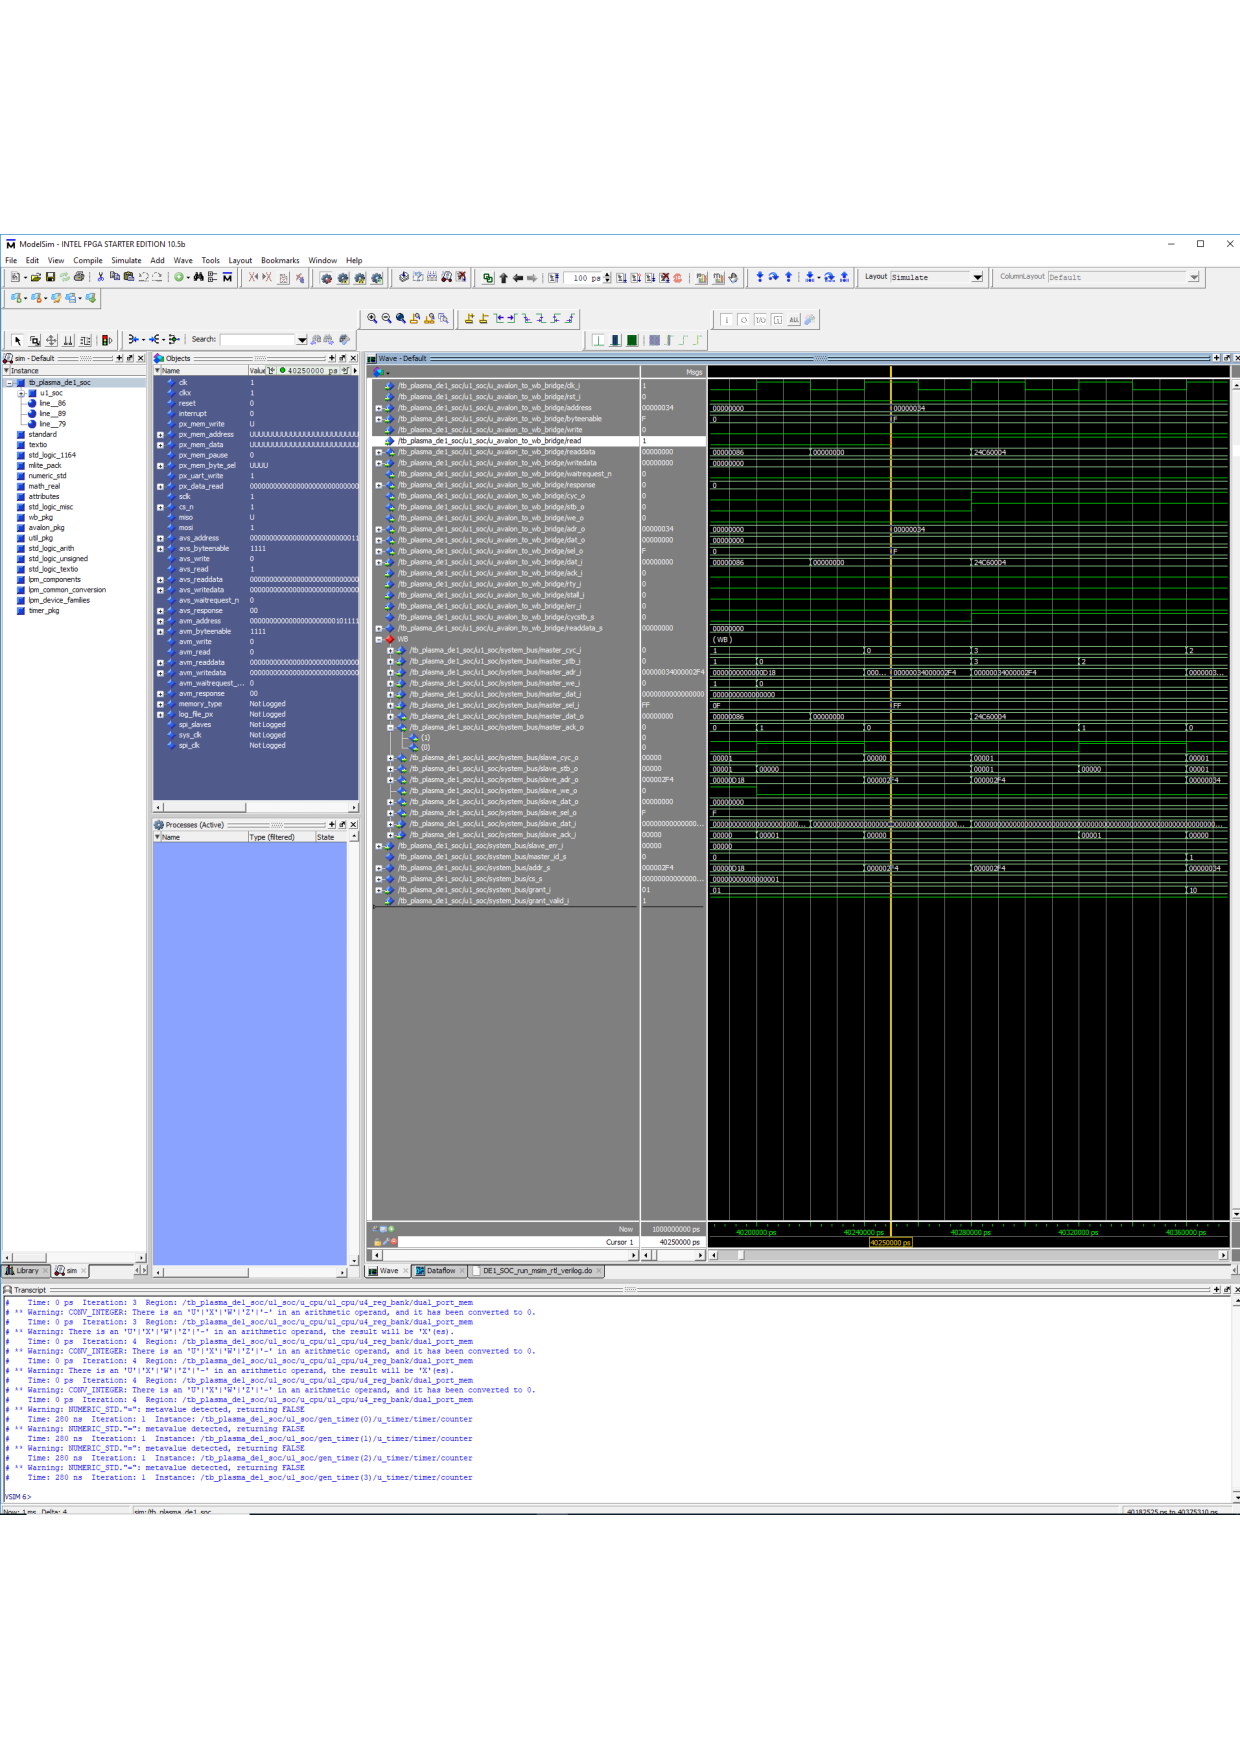
\includegraphics[width=\textwidth]{images/modelsim}
		\caption{Mentor Graphics Modelsim}
		\label{fig:modelsim}
	\end{subfigure}
	\caption{Quartus Anwendungen}
	\label{fig:quartus_apps}
\end{figure}

\section{SoC FPGA Embedded Development Suite (SoC EDS)}
Um Software für \gls{ARM}-basierte eingebettete Systeme entwickeln zu können, wird eine weitere Entwicklungsumgebung benötigt.
 
Genau so wie Quartus Prime ist SoC EDS nach einer Registrierung kostenfrei im Downloadportal\footnote{\url{http://fpgasoftware.intel.com/soceds/18.0/?edition=standard}} von Intel verfügbar. 

Folgende Anwendungen werden in dieser Bachelorarbeit verwendet:
\begin{easylist}[itemize]
	& Cross-Compiler für die \gls{ARM}-Architektur
	& Devicetree Compiler
	& \gls{BSP}-Editor
\end{easylist}